% !TeX spellcheck = en_GB
\documentclass[a4paper]{report}
\usepackage[T1]{fontenc}
\usepackage[utf8]{inputenc}
\usepackage[english]{babel}
\usepackage{geometry}
\usepackage{graphicx}
\usepackage{subfig}
\usepackage{fancyvrb}
\usepackage{tikz}
\usetikzlibrary{calc}

\usepackage{color}
\usepackage{listings}
\lstset{ %
	language=C++,                % choose the language of the code
	basicstyle=\footnotesize,       % the size of the fonts that are used for the code
	numbers=left,                   % where to put the line-numbers
	numberstyle=\footnotesize,      % the size of the fonts that are used for the line-numbers
	stepnumber=1,                   % the step between two line-numbers. If it is 1 each line will be numbered
	numbersep=5pt,                  % how far the line-numbers are from the code
	backgroundcolor=\color{white},  % choose the background color. You must add \usepackage{color}
	showspaces=false,               % show spaces adding particular underscores
	showstringspaces=false,         % underline spaces within strings
	showtabs=false,                 % show tabs within strings adding particular underscores
	frame=single,           % adds a frame around the code
	tabsize=2,          % sets default tabsize to 2 spaces
	captionpos=b,           % sets the caption-position to bottom
	breaklines=true,        % sets automatic line breaking
	breakatwhitespace=false,    % sets if automatic breaks should only happen at whitespace
	escapeinside={\%*}{*)}          % if you want to add a comment within your code
}

\geometry{a4paper,top=2.5cm,bottom=2.5cm,left=3cm,right=3cm,%
	heightrounded,bindingoffset=5mm}
\begin{document}
	
\begin{titlepage}

	\begin{tikzpicture}[overlay,remember picture]
		\draw[line width=4pt]
		($ (current page.north west) + (1cm,-1cm) $)
		rectangle
		($ (current page.south east) + (-1cm,1cm) $);
		\draw[line width=1.5pt]
		($ (current page.north west) + (1.2cm,-1.2cm) $)
		rectangle
		($ (current page.south east) + (-1.2cm,1.2cm) $);
	\end{tikzpicture}
	
	\begin{center}
		\textup{\large  \textbf{University of Pisa}\\[0.5cm]\textbf{\large M.Sc IN COMPUTER ENGINEERING}}
		
		%---------------------------------Figure------------------------------
		\vspace{\stretch{1}}
		\begin{center}
			\begin{figure}[h]  %h means here other options t , b, p, etc.
				\centering
				
\includegraphics[width=0.3\linewidth]{./img/unipi.png}
			\end{figure}
		\end{center}
		
		%----------------------------
		\begin{LARGE}
			{\textbf {"LINEAR FEEDBACK SHIFT REGISTER" }}\end{LARGE}\\[1cm]
		\textit{AUTHOR}\\[0.1cm]
		\begin{Large}
			\textbf{Francesco Iemma}\\[0.1cm]
		\end{Large}
		
		
		\vfill
		\vspace{\stretch{2}}
		\textbf{Academic Year: 2020/2021}
	\end{center}

\end{titlepage}

%\title{\Huge{Linear Feedback Shift Register}}
%\author{\Large{Francesco Iemma}}
%\date{Academic Year 2020/21}
%\maketitle
\tableofcontents

\chapter{Introduction}
The Linear Feedback Shift Register (LFSR) is a shift register \footnote{A shift register is a sequential logic circuit made up of  chain of flip flops, for each rising edge of the clock the value of each flip-flop is shifted to the next flip-flop} in which some bits are manipulated and fed back to the input in order to generate, thanks to the shifting, a sequence of bits. So we can say that its input is the output of a linear function of its previous state.

\noindent The initial value of the LFSR is the so-called seed and it affects the stream of bits generated by the LFSR. However, this stream is not (obviusly) really random because the number of possible states is finite and the stream of bits is determined by its current or previous state and, moreover, it is possible to compute the bit generated knowing the seed and the feedback function.
\noindent Anyway if the feeback function is well-choosen then the LFSR can produce a sequence of bits that appears random and which has a very long cycle, so this means that the output starts to repeat the generated numbers after a very long time. So we can assume, at least within a cycle, that it generates random numbers. For this reason the sequences generated from an LFSR are called pseudo-random.

\section{Algorythm Description}
In order to understand the LFSR algorythm we need to discuss about the \emph{feedback function}: it is the function which describes the way in which some spefic bits of the shift register are manipulated and then fed back to the input. Usually the arrangment of the inputs of the feedback function is represented as polynomial mod 2. In our case the feedback polynomial is:
\[1+x^{11}+x^{13}+x^{14}+x^{16}\]
Analysing the polynomial we can understand how LFSR works. In particular the feedback polynomial indicates which bits of the shift register affects the next state, these are called \emph{taps}.
In most cases the way in which the taps affect the next state is using XOR gates (but also XNOR gates can be used).

\noindent Now let's assume that we have an LFSR with a length of N and see how it works. At the starting state in the LFSR we have the seed. Then the feedback logic starts to work and the bit released from this logic is the new $0^{th}$ bit and the others bits are shifted by one to the right and due to the shift the previous last bit, i.e. the $(N-1)^{th}$ which has become\footnote{with $N^{th}$ we indicate the bit which is out of the LFSR. A shift register with a length of N has N bits and so its bits are the ones in the interval [0, N-1], the  $N^{th}$ doesn't exist but it's a way to indicate the "overflow" bit.} the $N^{th}$, will be the output of the LFSR.

\noindent In a more formal way (let's assume $b'_i$ the i-th old bit, $b_i$ the i-th new bit, N the length of LFSR with $N>0$, $T$ the set which contains the indexes of the taps and $y$ the function which represents the feedback logic) I can say:
\begin{itemize}
	\item $b_0 = y(b'_j, ..., b'_k)$ where  $j, ..., k \in T$
	\item $b_i = b'_{i-1}$  for $1\leq i<N$
	\item $output = b'_{N-1}$
\end{itemize}

\noindent The taps in our case are the bits 11, 13, 14, 16 (we can recognize them gazing to the exponents of \emph{x} in the feedback polynomial) so this means that the inputs of the feedback logic are these. And so in our previous notation (considering that we start to count from 0) we will have $T=\{10, 12, 13, 15\}$.

\noindent In the following image it's possible to see a logic representation of a generic LFSR.
\begin{figure}[htbp]
	\centering
	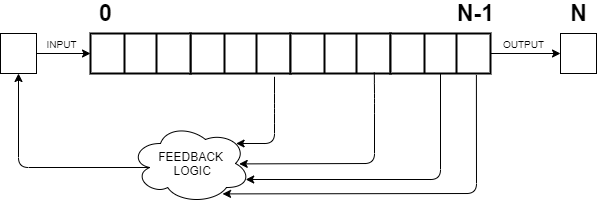
\includegraphics[scale=0.5]{img/LFSR-functionality.png}
	\caption{Logic representation of a LFSR}
\end{figure}
\section{LFSR's Properties}
Now let focus on a particular type of LFSR which has an interesting property, this is the so-called maximum-length LFSR. An LFSR is a maximum-length one, if and only if, the feedback polynomial is primitive and so it's necessary that:
\begin{itemize}
	\item The number of taps is even
	\item The taps values are coprime
\end{itemize}
The property of a maximum-length LFSR is the following: if its length is N then it will assume all the possible $2^N-1$ states (the state with all 0 is excluded because otherwise it will stop).

\noindent Others properties for generic LFSRs are:
\begin{itemize}
	\item As we can saw previously, the output is deterministic, in fact it's possible to compute it starting to the current state
	\item The state with all zeroes is not allowed, for this reason even a maximum-length LFSR cannot generate a sequence of $2^N$ states
\end{itemize}
It's important to point out that even if the output is deterministic the LFSRs are spreadly used, this happens because some techniques can be adopted to resolve this issue, for example giving an irregular clock to the device or manipulating the output stream with some non-linear combination of two or more bits extracted from this stream.

\section{Possible Applications}
LFSRs are spreadly used in a lot of fields. Let's see the most important ones:
\begin{itemize}
	\item They are used in Criptograhpy as pseudo-random number generators for stream-chipers (especially in military applications). In this field it's very important to resolve the issue about the deterministic behaviour of the LFSR in order to avoid possible attacks, some possible strategies are the ones seen in the previous section.
	\item They are used in Communication, for example in the Global Position System (GPS) and also in radio-jamming in order to generate a pseudo-random noise. Then another application in this field is for scrabbling, the bits produced from an LFSR are combined with the data bit in order to have a convenient stream of data that ensures good properties and better performance from the viewpoint of the modulator/demodulator. Then it is also used in CRC (Cyclic Redundancy Check).
	\item They are used in Electronics in order to do a pseudo-random testing of a circuit in order to test "all" possibile inputs of the circuit (in fact this technique is also called pseudo-exhaustive testing)
\end{itemize}


\section{Possible Architectures}
There are two type of possible LFSR's architectures:
\begin{itemize}
	\item Fibonacci LFSR (also called "Many-To-One architecture", because from "many" bits you obtain "one" bit that is the new input bit)
	\item Galois LFSR (also called "One-To-Many architecture", because from "one" bit - that is the last one and also the output - you obtain "many" bits that are the ones which are in positions next to the taps)
\end{itemize}
\begin{figure}[htpb]
	\centering
	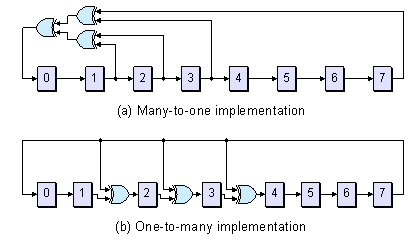
\includegraphics[scale=0.9]{img/architectures.png}
	\caption{LFSR Architectures - Source: www.eetimes.com}
\end{figure}
\subsection{Fibonacci LFSR}
The Fibonacci LFSR is the simplier possible architecture for an LFSR  and it is also the standard one, basically the generical things said so far about LFSRs describe the Fibonacci LFSR. In fact, for instance, we can observe that the figure 1.2.(a) and the figure 1.1 are indeed the same figure with the difference that the 1.1 is a logic representation and so the gates have not been drawn (they are in the so-called "Feedback Logic").
\subsection{Galois LFSR}
The Galois LFSR is an alternative architecture for LFSR, from the point of view of the output it's, more or less\footnote{A time offset is present and if some techniques are not adopted (the bit positions must be counted in the opposite direction of the shift) then one output is the reverse of the other one. In our case we neglect this difference because in any case the Galois is indeed a LFSR}, equivalent to Fibonacci one (the output of a Galois it's the same of a Fibonacci) but indeed they are internally different. On the rising edge of the clock, all bits that are not taps are shifted unchanged to the right by one position. Instead the taps are XORed with the previous last bit and the output of this XOR operation goes to the next bit on the right. In a more formal way we can write (let's assume $b'_i$ the i-th old bit, $b_i$ the new i-th bit, N the length of LFSR with $N>0$, $T$ the set which contains the indexes of the taps):
\begin{itemize}
	\item $b_0 = b'_{N-1}$
	\item $b_{i+1} = b'_i$ with $i\notin T$ , $0\le i < N-1$
	\item $b_{j+1} = XOR(b'_{N-1} , b_j)$ with $j \in T$ , $0\le j < N-1$
	\item $output = b'_{N-1}$
\end{itemize}
\subsection{Comparison and Critical Path}
The Galois architecture has a big advantage with respect to Fibonacci one. In fact in the latter there is a chain of XOR gates and the XOR operations must be done in serial and it cannot be done in parallel. Furthermore, the propagation time of this chain is not negligible. On the other hand, in the Galois implementation, the XOR operations can be done in parallel and the propagation time regard a single gate (not a chain as in the Fibonacci's case). So the propagation time of Galois implementation is lesser than the Fibonacci one, this means that with this architecture we can achieve a faster clock frequency.
In our case we have four taps, so if we assume that we have only XOR gates with two inputs and each one has a $t_{propagation_{i}} = x$ we are in the following situation:
	\begin{itemize}
		\item Fibonacci: we have to use three XOR gates (installed as we can see in the following image) and so the minimum clock period $T$ is equal to $T = t_{propagation_{1}} + t_{propagation_{2}} = 2x$. Then the maximum frequency achievable is $f=1/T=1/2x$. If $x=4ns$ then $f = 125 MHz$
		\begin{figure}[htpb]
			\centering
			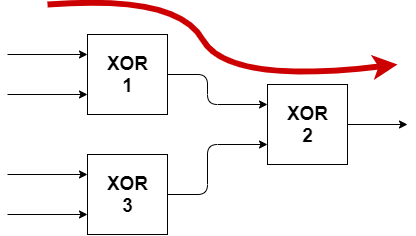
\includegraphics[scale=0.5]{img/XOR chain.png}
			\caption{Critical path (in red) related to XOR gate in Fibonacci with 4 taps}
		\end{figure}
		\item Galois: also in this case we use three XOR gates, but in this case each one is installed between two flip-flop so the critical path is made up of one gate. Then $T = t_{propagation_{1}} =x$ and so $f = 1/T = 1/x$. If $x=4ns$ then $f = 250 MHz$.
			\begin{figure}[htpb]
			\centering
			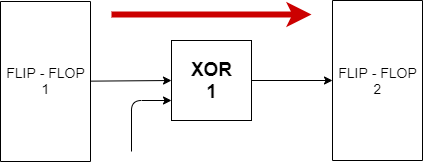
\includegraphics[scale=0.5]{img/XORtp.png}
			\caption{Critical path (in red) related to XOR gate in Galois}
		\end{figure}
	\end{itemize}
\noindent We can see that in this case $f_{Galois}=2f_{Fibonacci}$ but if the number of taps increase we have a larger difference, for example with $NumTaps = 8$ I have $f_{Galois} = 3f_{Fibonacci}$, with $NumTaps=16$ then $f_{Galois} = 4f_{Fibonacci}$. So if $NumTaps$ is $2^a$ then $f_{Galois} = af_{Fibonacci}$.

\noindent This results shown as the Galois implementation is better from the viewpoint of the maximum clock frequency.

\noindent This difference is bigger when the number of taps grows, but in most applications this difference is not so evident as in the example shown and, at the end of the day, the performance are more or less the same. For example if we use XOR gate with more inputs than two, the $t_{propagation}$ of Fibonacci is less than the one in the case of a cascade of XOR with two inputs. So the relation with Galois is not so unbalanced. Then in some FPGA are used LUTs that support 6 input logic function, so using a XOR with two inputs or a XOR with six is basically the same.

\noindent Indeed, theoretically speaking, the difference in performance between the two implementations exists, and so in the following report it will be treaten the implementation in VHDL of an LFSR with Galois architecture and then its testing and its practical realization obtained by programming the ZyBo Board with Xilinx Vivado. 

\chapter{Architecture Description}
As we discussed in the previous chapter, we will implement a Galois LFSR. Let's see the necessary devices to implement it.
In order to implement a memory element I need a D Flip-Flop with set and reset. In fact we need to initialize each memory element to the seed value, so the i-th flip flop will be initialize with the i-th bit of the seed.
The aim of the implementation is to have a functional LFSR, but another aim is also having a customizable LFSR. In order to do this we have to add a circuit to change (or not) the input of a simple flip-flop, we call this circuit \emph{tap circuit}. It will allow to set the taps, changing a proper input of the LFSR.
\section{D Flip-Flop with tap circuit}
Assume that we have the i-th flip-flop and the j-th (with $j = i +1$). If $i$ is a tap then its output must be XORed with the $N-1$ bit, otherwise the output of $i$ goes unchanged to the input of $j$. So we have to implement the following logic function (described using a pseudo-code and assuming that $feedback$ is the $N-1$ bit):
\begin{lstlisting}
	void logicFunctionOmega(isTap_i, feedback)
	{
		if(isTap_i==true)
			input_j = xor(output_i,feedback);
		else
			input_j = output_i;
	}
\end{lstlisting}
Now we have to translate this logic function from this pseudo-code to logic gates.
But, before doing this, we need to point out some concepts:
\begin{itemize}
	\item $isTap_i$, $feedback$ and $output_i$ are bits. We will use the following convention: $isTap_i$ is true if it is 1, it is false when it is 0.
	\item We know that the neutral element for the XOR is the 0 (A and B are the inputs of XOR: if B is 0 then A passes the gate unchanged), in fact the truth table for the XOR is:
	\begin{figure}[htpb]
		\centering
		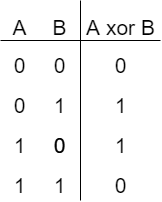
\includegraphics[scale=0.6]{img/XORtruthTable.png}
		\caption{XOR Truth Table}
	\end{figure} 
\end{itemize}

\noindent After fixed these points we can implement our function, let's call it $\Omega$ and let see what is the expected truth table (see figure 2.2).

\begin{figure}[htpb]
	\centering
	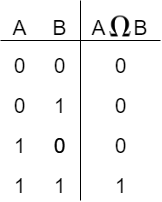
\includegraphics[scale=0.6]{img/ANDtruthTable.png}
	\caption{$\Omega$ Truth Table. A is $isTap_i$ and B is $feedback$}
\end{figure}

\noindent Remember that the output must be equal to B ($feedback$) if A($tap_i$) is equal to 1, otherwise it must be equal to the neutral element of the xor, so 0.

\noindent We can easily recognize that the "mysterious" logic function $\Omega$ is indeed the AND gate.
So the logic block diagram of a flip-flop with the tap circuit is the following:
\begin{figure}[htpb]
	\centering
	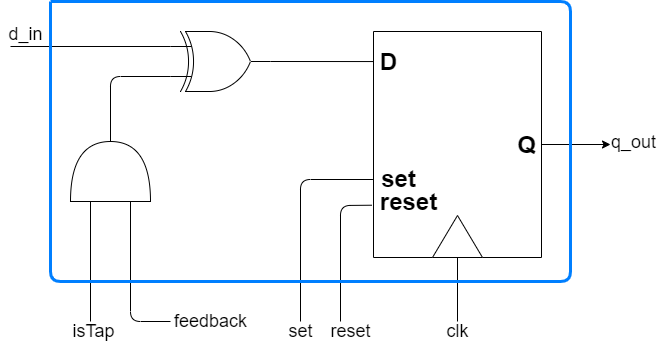
\includegraphics[scale=0.6]{img/FF_tap_circuit.png}
	\caption{Logic block diagram of a D Flip-Flop with set/reset and tap circuit.}
\end{figure}

\section{LFSR Implementation}
Once we have the D Flip-Flop with the tap circuit if we want to implement a LFSR with a length of N, we need N D Flip-Flop with tap circuit.
\begin{figure}[htpb]
	\centering
	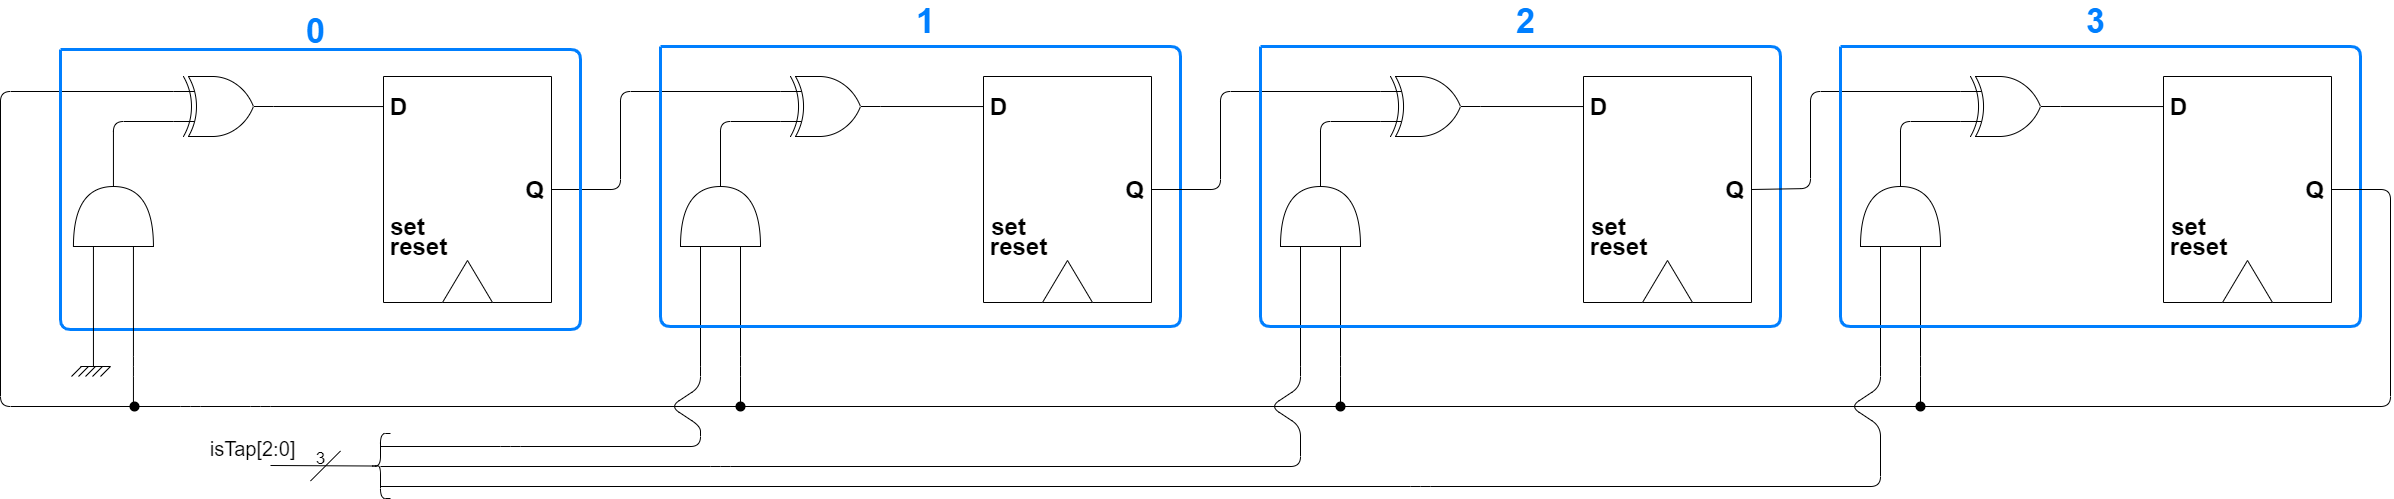
\includegraphics[scale=0.19]{img/LFSR_logic_block.png}
	\caption{Implementation of a LFSR (length of 4) with D Flip-Flop with tap circuit. (For simplicity we neglect the links for clock and set/reset)}
\end{figure}

\noindent It's important to do some observations about this implementation.
\begin{itemize}
	\item The first flip flop (the $0^{th}$) is a particular one. Its input port "isTap" must be linked to the ground (it must be always 0) because doesn't exist a flip flop before the zero one.
	\item The initialization of the flip-flops is ensured by the basic D Flip-Flop linking the set port of the $i^{th}$ flip-flop to $seed[i]$ (this is not shown in figure 2.4)
\end{itemize}

\section{Input/Output and Overall}
Abstracting from the internal details it's possible to describe the LFSR as in the image 2.5.
\begin{figure}[htpb]
	\centering
	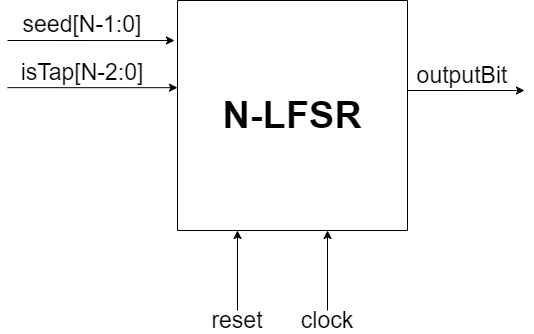
\includegraphics[scale=0.5]{img/LFSR-overall.png}
	\caption{Logic block diagram of a LFSR with a length of N.}
\end{figure}

\noindent Let's analyse the input/output ports:
\begin{itemize}
	\item \emph{seed[N-1:0]}: it contains the initialization value of the LFSR (the so-called seed). As we said previously the $i-th$ set port of the flip-flop will be connected to $seed[i]$.
	\item \emph{isTap[N-2:0]}: it indicates which are the taps. Its length is N-1 because there is no flip-flop before the $0^{th}$ flip-flop and so its isTap port will be connected to the ground (zero).
	\item \emph{reset}: the reset in common for all flip-flops.
	\item \emph{clock}: the clock in common for all flip-flops.
	\item \emph{outputBit}: the bit that is the result of the LFSR's algorithm.
\end{itemize} 
Let's sum up the operations done by the LFSR:

\noindent The LFSR is programmable, because once we have fixed the length N it can works with any polynomial feedback because of \emph{isTap[N-2:0]}. Then it's also possible to initialize, at the reset, the shift register using \emph{seed[N-1:0]}. Then, when all these signal are given to the device, it start to work and to produce a pseudo-random sequence of bits.
\chapter{VHDL Code}
In this section we will see the VHDL code for all the devices seen previously: starting from the basic ones, that are necessary to implement an LFSR, to arrive at the LFSR itself.
\section{D Flip-Flop with Set/Reset}
The basic device needed for the LFSR is a D Flip-Flop wit Set/Reset.
\lstset{ %
	language=VHDL}
\begin{lstlisting}
	-- D Flip-Flop with Set/Reset
	library ieee;
	use ieee.std_logic_1164.all;
	
	entity dff is
		port(
			clk		:	in 	std_logic;
			reset	:	in 	std_logic;
			set 	:	in 	std_logic;
			d 		:	in 	std_logic;
			q 		:	out std_logic
		);
	end dff;
	
	architecture rtl of dff is
	begin
		dff_p:process(reset,clk,set)
	begin
			--if reset='0' then 	-- Standard Reset Polarity 
			if reset='1' then  		-- ZyBo Board Reset Polarity
				q <= set;
			elsif(rising_edge(clk)) then
				q <= d;
			end if;
		end process;
	end rtl;
\end{lstlisting}
The behaviour of this device is very simple, at the initialization phase (when reset is 0 if we consider the standard reset polarity) the output is initialized with the set value. Then in the normal case the output follow the input and it is update at each rising edge of the clock.
An important note is that the reset polarity will be changed afterwards for synthesis reasons that will be explained afterwards in chapter 5.

\section{D Flip-Flop with Set/Reset and Tap Circuit}
The memory cell which maintains a bit within the LFSR is the D-Flip-Flop with Set/Reset and tap circuit that implements the characteristic features of the LFSR which differentiates it from a simple shift register.
\begin{lstlisting}
	-- D Flip-Flop with Set/Reset and tap circuit
	library ieee;
	use ieee.std_logic_1164.all;
	
	entity dff_tap_circuit is
		port(
			clk				:	in 	std_logic;
			reset 		:	in 	std_logic;
			set				:	in 	std_logic;  -- initialization input (necessary for seed
																	-- initialization)
			d_in			:	in 	std_logic;	
			isTap			:	in 	std_logic;	-- it indicates if the input must be changed
																	-- (it does if the previous ff is a tap)
			feedback	:	in 	std_logic;  -- it is the feedback bit (the N-1 bit of 
																	-- the LFSR)
			q_out			:	out std_logic
		);
	end dff_tap_circuit;
	
	
	architecture rtl of dff_tap_circuit is
	component dff is
		port(
			clk		:	in 	std_logic;
			reset :	in 	std_logic;
			set		:	in 	std_logic;
			d 		:	in 	std_logic;
			q 		:	out std_logic
		);
	end component;
	
	signal new_d : std_logic; -- signal that is the result of the logic (XOR+AND)
														-- and it is the dff input
	begin
		internal_dff : dff
		port map(
			clk 	=> clk,
			reset	=> reset,
			set 	=> set,
			d 		=> new_d,
			q 		=> q_out
		);
		
		new_d <= d_in xor (isTap and feedback);
	
	end rtl;
\end{lstlisting}
This device acts as the previous, the only difference is the addition of the tap circuit which is described in the row 41.

\section{LFSR}
Now we see the way in which we have to aggregate the previous devices in order to implement an LFSR.

\noindent We use (0 to N) instead of (N downto 0) in the declaration of the standard logic vectors for isTap and seed, because they are not numbers but they indicate positions, so the left-most bit is the one for the $0^{th}$ flip-flop and so in order to access it I would like to use the following notation: \emph{vector(0)} and not this \emph{vector(N-1)}. To achieve this aim I have to use the keyword \emph{to} instead of \emph{downto}.
\begin{lstlisting}
	-- LinearFeedbackShiftRegister
	library ieee;
	use ieee.std_logic_1164.all;
	
	entity lfsr is
		generic (Nbit : positive := 16);
		port(
			clock		:	in 	std_logic;
			reset 		:	in 	std_logic;
			isTap		: 	in 	std_logic_vector(0 to Nbit-2);
			seed		:	in 	std_logic_vector(0 to Nbit-1);
			outputBit	: 	out std_logic;
			-- Debugging: it's necessary to stop the simulation in ModelSim.
			-- But can be useful also in normal application.
			state		: 	out std_logic_vector(Nbit-1 downto 0)
		);
	end lfsr;
	
	
	architecture rtl of lfsr is
		component dff_tap_circuit is
			port(
				clk				:	in 	std_logic;
				reset 		:	in 	std_logic;
				set				: 	in 	std_logic; 	-- initialization input (necessary for
																			-- seed initialization)
				d_in			:	in 	std_logic;	
				isTap			:	in 	std_logic;	-- it indicates if the input must be changed
																		-- (it does if the previous ff is a tap)
				feedback	:	in 	std_logic;  -- it is the feedback bit (the N-1 bit of
																		-- the LFSR)
				q_out			:	out std_logic
			);
		end component;
		
		signal lastBit : std_logic;							-- Last bit of the LFSR, it is the
																						-- feedback bit and also the output
		signal intercon : std_logic_vector(0 to Nbit-2);	-- Interconnections among
																											-- flip-flops
	begin
		GEN:for i in 0 to Nbit-1 generate
			FIRST: 	if i = 0 generate
			FF1 : dff_tap_circuit port map(clock, reset, seed(i), lastBit,'0', lastBit,intercon(i));
			end generate FIRST;
			
			INTERNAL:	if (i>=1) and (i<Nbit-1) generate
			FFI : dff_tap_circuit port map(clock, reset, seed(i), intercon(i-1), isTap(i-1), lastBit, intercon(i));
			end generate INTERNAL;
			
			LAST:	if i=Nbit-1 generate
			FFL : dff_tap_circuit port map(clock, reset, seed(i), intercon(i-1), isTap(i-1), lastBit, lastBit);
			end generate LAST;
		end generate GEN;
		
		state <= intercon & lastBit;
		outputBit <= lastBit;
	end rtl;
\end{lstlisting}
In the next chapter we will see the strategies to test this device and to ensure that it works as a Linear Feedback Shift Register.
\chapter{Test-Plan}
In this chapter we will test the LFSR implemented in VHDL in the previous chapter. In order to accomplish this aim we will start testing the basic elements of the implementation up to the final LFSR. The tests performed and explained will be:
\begin{itemize}
	\item Test of a simple D-Flip-Flop
	\item Test of a D-Flip-Flop with tap circuit
	\item Test of the LFSR with isTap inputs to 0, so it's a simple shift register
	\item Final test of the LFSR using a C++ program which does in software what we implemented in hardware using VHDL
\end{itemize}
In some cases only a portion of the code will be shown, for the full code see files in LFSR/hdl/tb/

\noindent When we indicate the number of clock cycles we don't consider the clock cycles of the reset state. So "after $x$ clock cycles" means "after $x$ clock cycles counted from when reset is not active.  

\section{D-Flip-Flop Test}
In order to test the simpler device (dff) we give as input 0, so the expected result is that until we change the input the output remains 0.
\begin{lstlisting}
	dff_process : process(clk_tb,reset_tb)
	variable t : integer := 0;
	begin
		if(reset_tb='0') then
			t:=0;
			d_tb <= '0';
		elsif (rising_edge(clk_tb)) then
			case(t) is
				when 5 => d_tb <= '1';	
				when 10 => end_sim <= '0';	
				when others => null;		
			end case ;
			t:=t+1;
		end if;
	end process;
\end{lstlisting}
The test consist in given 0 at the reset and then after 5 clock cycles change the input to 1.
\begin{figure}[htpb]
	\centering
	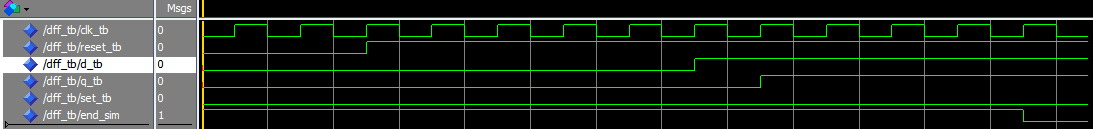
\includegraphics[width=.6\textheight, height=.125\textheight]{img/tb/wave_dff_test.png}
	\caption{Simulation of dff test-bench using ModelSim}
\end{figure}

\noindent As we can see in the image flip flop works as we expected:
\begin{itemize}
	\item At the reset the output is equal to the value of the set
	\item The ouput remains unchanged until the input is 0, when the input change to 1 (5 clocks after the end of reset) also the output follows it after a clock cycle.
\end{itemize}

\section{D-Flip-Flop with Tap Circuit Test}
Now we want to test also the flip-flop with tap circuit, if the input isTap is 0 the flip-flop works exactly as the previous one. Instead if isTap is 1 and the feedback bit is 1 too then it's like an inverter (because the xor at the input has always an input at 1).
\begin{lstlisting}
	dff_process : process(clk_tb,reset_tb)
	variable t : integer := 0;
	begin
		if(reset_tb='0') then
			t:=0;
			isTap_tb <= '0'; 	-- It's a normal dff
			feedback_tb <= '1';
			d_tb <= '0';
		elsif (rising_edge(clk_tb)) then
			case(t) is
				when 5  => d_tb <= '1';		
				when 10 => isTap_tb <= '1'; d_tb <='0';	
				when 15 => d_tb <='1';	
				when 20 => end_sim <= '0';
				when others => null;	
			end case ;
			t:=t+1;
		end if;
	end process;
\end{lstlisting}
So we expect that for the first 10 clock cycles after reset the waves are the same of the previous case and then they present a inverter-like behaviour.
\begin{figure}[htpb]
	\centering
	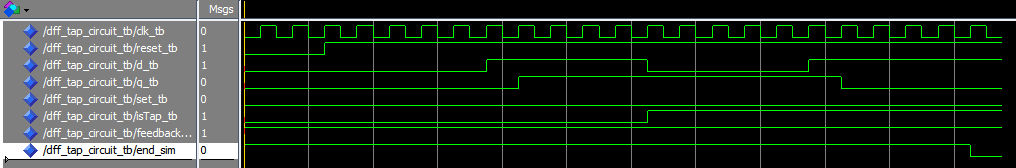
\includegraphics[width=.6\textheight, height=.125\textheight]{img/tb/wave_dff_tap_circuit_test.png}
	\caption{Simulation of test-bench of dff with tap circuit using ModelSim}
\end{figure}

\noindent From the figure 4.2 we can say that the behaviour is the one that we expect:
\begin{itemize}
	\item In the first 10 clock cycles (after the reset) the waves are the same of the dff case. This is right because in this period we have isTap to 0 and so the tap circuit is disabled
	\item When isTap goes to 1 the dff with tap circuit works as an inverter (remember that feedback is 1). In fact in this moment we can see that the output remains one even if the input goes from 1 to 0. This happens because the input goes to 0 so the output at the next clock cycle will became one but it is already one, then it remains 1.
	
	\noindent When the input goes to 1 (after 15 clock cycles), the output, after a clock cycle, goes to 0 as we expected. 
\end{itemize}

\section{LFSR as Shift Register}
If all bits of isTap are setted to 0 then we have a simple shift register because there are no taps. So this test consists in doing this and in controlling the proper work of this shift register.

\begin{lstlisting}
	lfsr_test_process : process(clk_tb,reset_tb)
	variable t : integer := 0;
	begin
		if(reset_tb='0') then
			t:=0;
			isTap_tb <= "000000000000000";
			seed_tb <= "0000101011000110";
		elsif (rising_edge(clk_tb)) then
			if actual_state=seed_tb and t=0 then
				t:=t+1;
			elsif actual_state=seed_tb and t=1 then
				end_sim <='0';
			end if;
		end if;
	end process;
\end{lstlisting}
We stop the simulation when the actual state of the shift register is equal to the initial one, hence we expect that the simulation ends after 16 clock cycles because the register has a length of 16 and so after this period each bit are shifted 16 times and so it has returned in the initial position.

\noindent The reason why we neglect the first time that th actual state is equal to the seed is because this happens at the initialization and if we consider this the first time then the simulation ends early.

\begin{figure}[htpb]
	\centering
	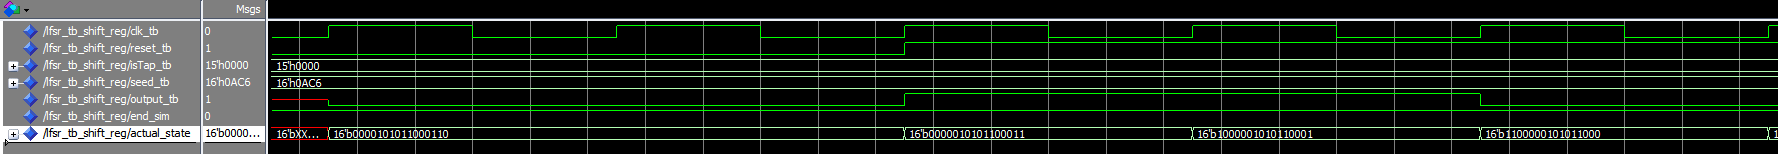
\includegraphics[width=.6\textheight, height=.1\textheight]{img/tb/wave_lfsr_as_shift_reg_test_bin.png}
	\caption{Part of the simulation of the test-bench of a lfsr setted as shift register}
\end{figure}

\noindent In the figure 4.3 we can see the initial part of the simulation, as we can see the first states of the device are the ones that we expect from a shift register.

\begin{figure}[htpb]
	\centering
	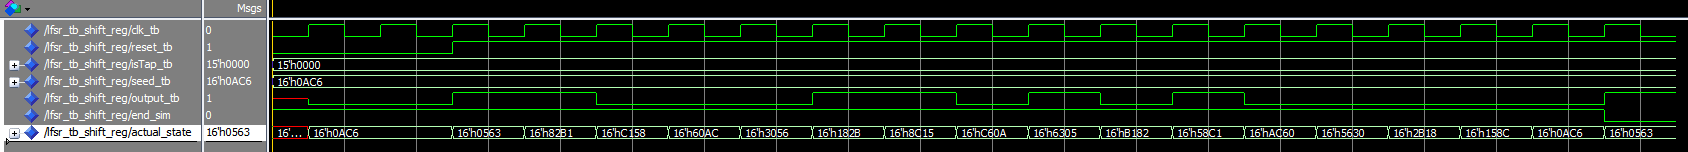
\includegraphics[width=.6\textheight, height=.1\textheight]{img/tb/wave_lfsr_as_shift_reg_test_hex.png}
	\caption{Complete simulation of the test-bench of a lfsr setted as shift register}
\end{figure}

\noindent In the figure 4.4 we can see the complete configuration (in order to have a more compact image the format of the state is hexadecimal). Here we can see that after the reset the shift register spends 16 clock cycles to reach its initial state as we expected.

\section{LFSR}
In order to prove the proper work of the LFSR we do a final test using a test-bench in VHDL and a C++ program. The program does in software the operations that are done in hardware by an LFSR. Both the test-bench and the program write their output on a file, the two file must be equal to ensure the correctness of the LFSR. Two script helps in doing this operations, one compiles and executes the C++ program, instead the other one compares the two output file using the UNIX tool \emph{diff}. The scripts work only in a UNIX-like environment.
\subsection{LFSR Test-bench}
\noindent The test-bench is like the previous one, but in this case the tap are setted at the following feedback polynomial: 
\[1+x^{11}+x^{13}+x^{14}+x^{16}\]
Then in terms of bit position the taps are: 10, 12, 13. Because of the fact that we start to count from 0. The bits 0 and 15 (i.e. the first one and the last one are always taps in a LFSR because the output is fed back to the input, but they are not taps in the sense that the must be XORed).
\begin{lstlisting}
	lfsr_test_process : process(clk_tb,reset_tb)
	variable t : integer := 0;
	begin
		if(reset_tb='0') then
			t:=0;
			isTap_tb <= "000000000010110";
			seed_tb <= "0000101011000110";
		elsif (rising_edge(clk_tb)) then
			-- The first time it's at the beginning and I have to neglect it
			if actual_state=seed_tb and t=0 then
				t:=t+1;
			-- The second time it's at the end and so I have to stop the sim
			elsif actual_state=seed_tb and t=1 then	
				end_sim <='0';
			end if;
		end if;
	end process;
	
	-- Process that write the output on a file
	write_file : process
	variable BUF : line;
	begin
		loop
			wait on clk_tb until clk_tb='1';
			if reset_tb='1' then
				WRITE(BUF,output_tb);
				WRITEline(OUT_LFSR,BUF);
			end if;
		end loop;
	end process;
\end{lstlisting}

\noindent The last process is in charge of writing the output on a file in order to compare it afterwards with the output of the C++ program.

\noindent The statement at row 21 means that the output is written in the file on the rising edge of the clock (it waits until the clock changes from 0 to 1). Then at row 22 the if statement is needed in order to avoid the print of the output during the reset state.

\subsection{C++ Test Program}
The C++ program follows the same approach of the VHDL implementation. It is a Galois LFSR implemented in software. Anyway the implementation is not very performing because the target of the program is to test an already implemented hardware LFSR and not to implement in the most efficient way an LFSR.  
\lstset{ %
	language=C++ }
\begin{lstlisting}	
	int main()
	{
		// Initialization value
		int seed[N] = {0,0,0,0,1,0,1,0,1,1,0,0,0,1,1,0}; 
		// Actual state of the LFSR
		int actual_state[N];
		// Reset Phase: actual state is initialized to the seed value
		for(int i = 0; i<N; i++)
			actual_state[i] = seed[i];
		do {
			// Feedback bit
			int lastBit = actual_state[N-1];
			// Next LFSR state
			int next_state[N];
			// Shift operation
			for(int i = 0; i<N; i++)
			{
				if(i!=0 && isTap(i-1))
					next_state[i] = xorFunction(actual_state[i-1],lastBit);
				else if(i==0)
					next_state[i] = lastBit;
				else
					next_state[i] = actual_state[i-1];
			}
			
			// The next state became the actual state
			for(int i = 0; i<N; i++)
				actual_state[i] = next_state[i];
			
			// Print the output
			cout << lastBit << endl;
		}while(!compare(actual_state,seed));
		
		/* Print the output of the last state (i.e. the first of the new cycle)
		 * This is necessary to emulate the effect of the end_sim
		 * in VHDL. When the condition in the while is true then
		 * the simulation ends but in the ModelSim simulation
	 	 * it ends after a clock (because end_sim goes to 0 after
	   * a clock cycle). So the output of the first state of the 
	 	 * new cycle must be considered*/
		cout << actual_state[N-1] << endl;
		return 0;
	}
\end{lstlisting}

\noindent Only the main is shown, for the complete code see \begin{Verbatim}
	/lfsr_cpp/lfsr_software.cpp
\end{Verbatim}
It's important to underline the statement at row 41. This statement is necessary in order to take into account the fact that the ModelSim simulation ends after a clock cycle, that is the period that the signal that is in charge of ending simulation needed to change from 0 to 1. More in the comment within the code.

\subsection{Helper Scripts}
The first script is in charge of compiling the code and redirecting the output in the file output.txt.
\lstset{ %
	language=sh }
\begin{lstlisting}	
	#!/bin/bash
	g++ lfsr_software.cpp -o lfsr
	./lfsr > output.txt
\end{lstlisting}

\noindent The second one is in charge of use the tool \emph{diff} to compare the output of the program and the output of the ModelSim simulation.
\begin{lstlisting}	
	#!/bin/bash
	# Check if there are differences between two file
	
	VAR=`diff output.txt ../LFSR/ModelSim/LFSR_test/fileout.tv`
	
	if [ -z "$VAR" ]
	then
		echo "OK - NO DIFFERENCES"
	else
		echo $VAR
	fi
	
	echo "Press a key to exit"
	read input
\end{lstlisting}

\noindent At row 6 the output of diff is controlled and the condition in the if statement return true if and only if the command return null (so it means that there are no differences between the two files). Otherwise it means that there are some differences and so these are shown.

\subsection{ModelSim Simulation}
The first step of the complete test is the ModelSim simulation performed with the test-bench seen at paragraph 4.4.1.
\begin{figure}[htpb]
	\centering
	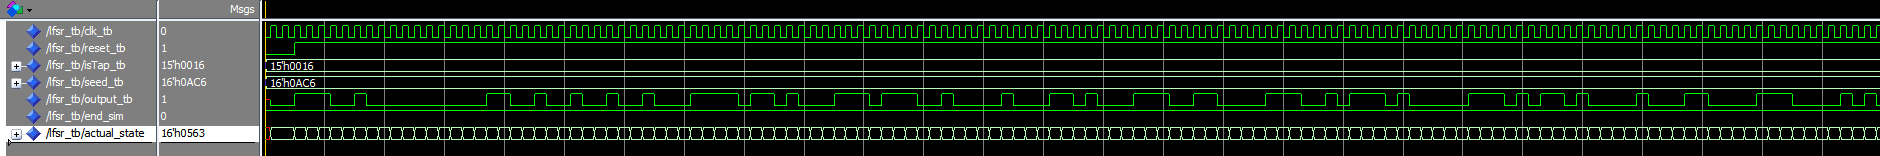
\includegraphics[width=.64\textheight, height=.09\textheight]{img/tb/wave_lfsr_test2.png}
	\caption{Part of the simulation of the lfsr test-bench}
\end{figure}

\noindent In the figure 4.5 is shown the output of the lfsr simulation as in the wave form. From this we can extract very poor information, in fact the only thing that we can say is that at the first view the output doesn't show a pattern and so maybe it can considered pseudo-random, but in order to be sure of this we have to check the output of this simulation with the C++ program output.

\subsection{Check The Simulation With C++ Program}
After the ModelSim simulation we have the output in the file at the following path:
\begin{Verbatim}
	/LFSR/ModelSim/LFSR_test/fileout.tv
\end{Verbatim}
Now we have to use the helper scripts.

\noindent The first thing to do is to go in the directory in which there are C++ program and scripts.
\begin{Verbatim}
	cd /lfsr_cpp/
\end{Verbatim}
Then we can execute the script which compiles and redirect the output of the program to the file output.txt
\begin{Verbatim}
	./run_lfsr.sh
\end{Verbatim}
If the console gives no error then the compilation and the execution are done successfully. So now we can check the two output using the proper script:
\begin{Verbatim}
	./check.sh
\end{Verbatim}
If the console returns
\begin{Verbatim}
	OK - NO DIFFERENCES
\end{Verbatim}
Then it means that the test is ended successfully and that the LFSR implemented in VHDL works in a proper way.
In the figure 4.6 we can see the output of the last steps in Linux console.
\begin{figure}[htpb]
	\centering
	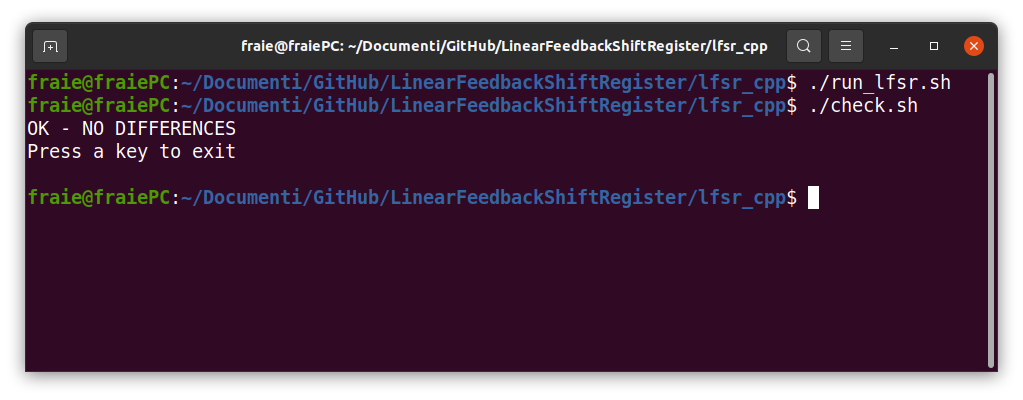
\includegraphics[scale=0.4]{img/tb/linuxConsoleExecution.png}
	\caption{Execution of the scripts in Linux console}
\end{figure}
\subsection{LFSR Test Conclusion}
For a complete test plan we have to test all the $2^{16}-1$ (Remember that the state with all 0 is not allowed) possible seeds and so we have to do $65535$ tests and comparisons. Only in this way we can be sure, without doubts, that the LFSR works properly. Anyway we do only some tests and we can say with a reasonable confidence that the LFSR works in a proper way.

\noindent In particular three tests are performed with the following seeds:
\begin{itemize}
	\item 0000101011000110 
	\begin{Verbatim}
	/lfsr_cpp/output.txt
	/LFSR/ModelSim/LFSR_test/fileout.tv
	\end{Verbatim}
	\item 1100101010100111
	\begin{Verbatim}
	/lfsr_cpp/output1.txt
	/LFSR/ModelSim/LFSR_test/fileout1.tv
	\end{Verbatim}
	\item 0000000000000110
	\begin{Verbatim}
	/lfsr_cpp/output2.txt
	/LFSR/ModelSim/LFSR_test/fileout2.tv
	\end{Verbatim}
\end{itemize}
Each test has been performed as the one previously explained and each one has given a successfully output.
\chapter{Logic Synthesis}
In this chapter we discuss the Logic Synthesis of the previously implemented LFSR, with Xilinx Vivado, for ZyBo Board (ZYNQ XC7Z010-1CLG400C).

\section{LFSR Wrapper}
In order to synthesize the LFSR on the FPGA we have to do some trade-offs. This because the ZyBo Board has only 4 push buttons and 4 slide switches as input. So we have to implement a wrapper that reduces the number of inputs of our LFSR.

\noindent Before the synthesis we have the following inputs\footnote{The clock is not considered because it is not an input given by the user}:
\begin{itemize}
	\item isTap: 15 bits
	\item seed: 16 bits
	\item reset: 1 bit
\end{itemize}  

\noindent So we would need 32 input ports and we have not them. To resolve this issue we do the following trade-offs:
\begin{itemize}
	\item The input for decide which bits are taps or not, is given by the wrapper and it is a pre-determined value (the same seen in test-plan, that is the one of the requirements).
	\item Only a part of the seed value is editable, this part will be connected with the 4 slides switches and a feedback of which slides are active, is given to the user using 4 leds provided by the board. The rest of the seed is pre-determined with a non-zero value, so even if the user doesn't change the slides, the LFSR works properly because in any case the seed is a non-zero value.
	
	\noindent
	So the seed will be \emph{userInput + 101011000110} (where + means concatenation).
	
	\item The reset value is connected with one of the push buttons. This means that we have to invert the polarity of the reset, because when a user pushes the button this means that a $V_{cc}$ to the reset is given (so reset is equal to 1 if the button is pushed, 0 otherwise), so the reset is asserted when the push buttons is pressed, only if the polarity of the reset is inverted. In order to resolve this issue, the polarity of the dff must be inverted.
\end{itemize}

\noindent Then we have to resolve also the issue about the output. In this case we have as output only a bit, so if we want to show the result on a screen we have to use the VGA output. In order to do this we can use 6 bits of DAC on the GRN channel. Thus, we assign the output bit to the less significant bit of these 6 and the others are setted to 0.

\noindent To see the wrapper VHDL code see the correspondent VHDL file:
\begin{Verbatim}
	/LFSR/hdl/src/lfsr_wrapper.vhd
\end{Verbatim}

\subsection{Wrapper Test}
\noindent Also the wrapper has been tested using the test-bench and the comparison with the C++ program. The wrapper test bench is in the path:
\begin{Verbatim}
	/LFSR/hdl/tb/lfsr_wrapper_tb.vhd
\end{Verbatim}

\noindent Some observations about it are needed:
\begin{itemize}
	\item The reset polarity is inverted in order to emulate the behaviour of the push buttons (as we can see in the figure 5.1).
	\begin{figure}[htpb]
	\centering
	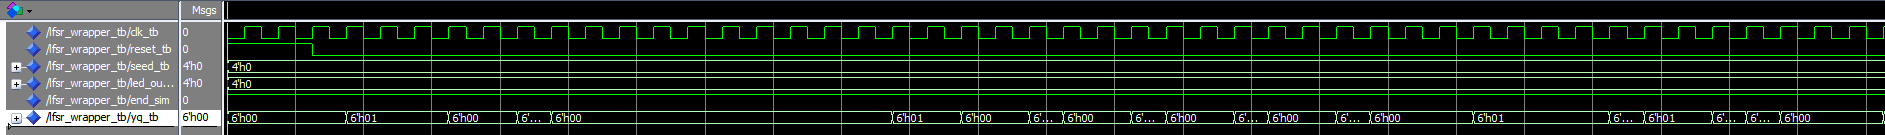
\includegraphics[width=.64\textheight, height=.09\textheight]{img/tb/wave_lfsr_wrapper_test.png}
	\caption{Part of the simulation of the lfsr wrapper}
	\end{figure}
	\item The output (only the LSB) is saved in a file in order to be compared with the C++ program output.
	\item Due to the fact that now there is no way to know the internal state of the LFSR we stop the simulation after 65536 clock cycles.
\end{itemize}
Then, after ModelSim simulation, we can use the scripts (changing the paths of the file) to check the simulation output file. The correctness of the wrapper implementation is ensured by the fact that the wrapper doesn't modify the job of the standard LFSR (that is emulated by the C++ program) because the simulation output file and the C++ output file have no differences.

\section{RTL Analysis}
The first step of Vivado workflow is to perform the RTL analysis of our device. The output of this step is a schematic of the LFSR.
\begin{figure}[htpb]
	\centering
	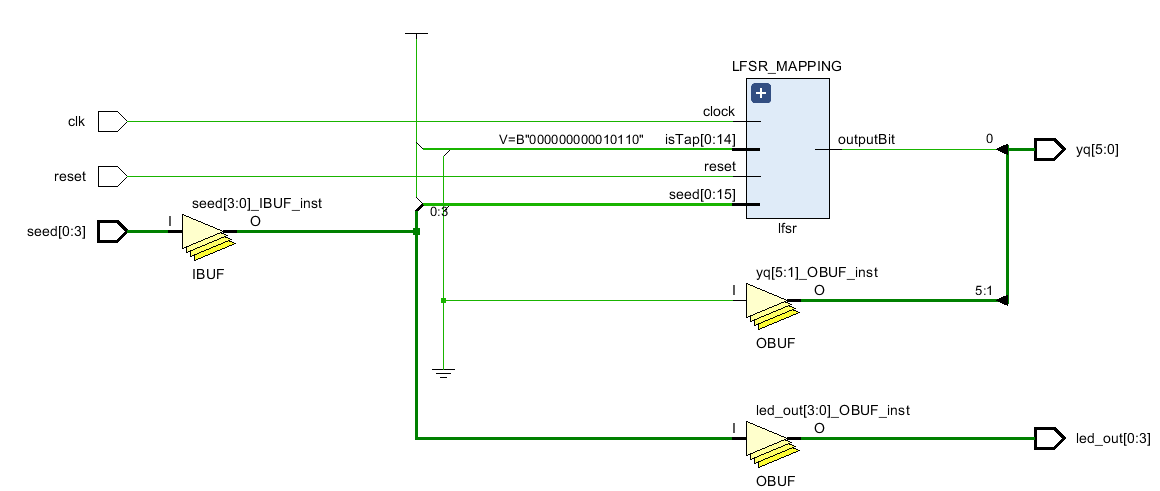
\includegraphics[scale=0.5]{img/vivado/rtl_analysis_schematic.PNG}
	\caption{RTL Analysis Schematic}
\end{figure}

\noindent In the figure 5.2 we can see the schematic, we can recognize the inputs and the outputs and the fact that some of them are initialized to constant values (the connections to ground and to power supply).

\begin{figure}[htpb]
	\centering
	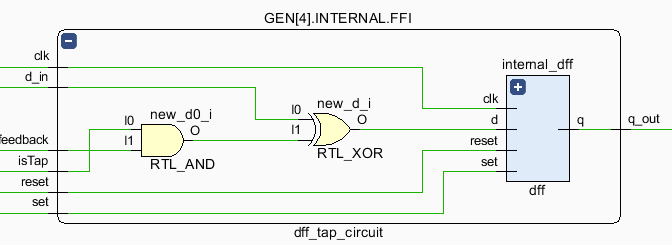
\includegraphics[scale=0.7]{img/vivado/detail_of_rtl_analysis.png}
	\caption{Detail of a D-Flip-Flop of RTL Analysis Schematic}
\end{figure}

\noindent In the figure 5.3 we can see the implementation in terms of logic gate. We can see also the critical path, in fact we can say that the critical path of the device, which determines the maximum clock frequency, is indeed the one that starts at the output of an internal flip-flop and ends at the input of the next one as we expect at the beginning in the design phase (for an in-depth view about the critical path and the design choises done see 1.4.3).

\noindent In order to explore this topic we have to say that in the latter quoted section we don't consider the fact that in order to have a programmable LFSR we have to add an AND gate. In any case the Galois implementation is the best because, if we want to implement a programmable Fibonacci LFSR, we have to use a demultiplexer before the feedback logic in order to select which bits are taps and must be manipulated, so the critical path would be more critical.

\begin{figure}[htpb]
	\centering
	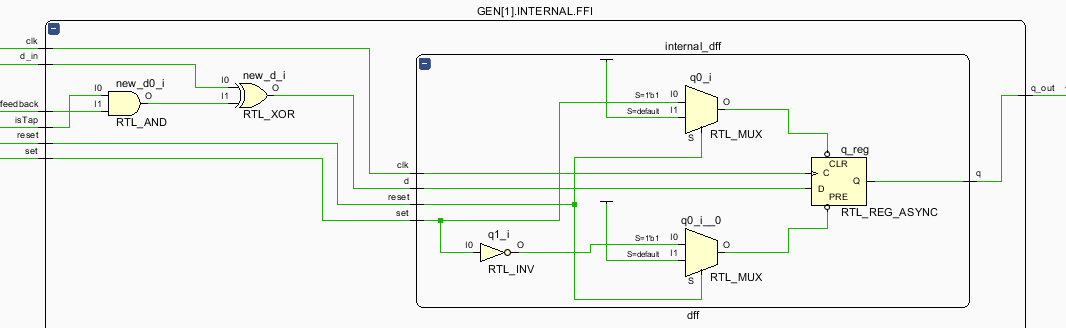
\includegraphics[scale=0.55]{img/vivado/detail_of_detail_of_rtl_analysis.png}
	\caption{Detail of a D-Flip-Flop with internal implementation (RTL Analysis Schematic)}
\end{figure}

\section{Synthesis}
With this second step we map our structure on the target technology.
\subsection{Clock Period Setting}
In this step we have to set the clock timing. We try to get a clock frequency of 125 MHz (8 ns). If we run the synthesis with this clock frequency we obtain the timing summary in figure 5.5.
\begin{figure}[htpb]
	\centering
	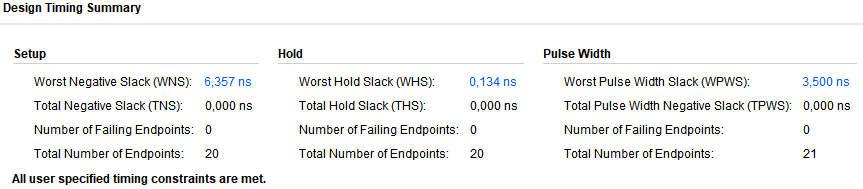
\includegraphics[scale=0.6]{img/vivado/timing_summary1.png}
	\caption{Design Timing Summary with period clock equal to 8 ns}
\end{figure}


\noindent We can see that the slack is 6,357 ns, so this means that our device can work at an higher frequency. So we edit the clock period to 5 ns. In this case we have a Worst Negative Slack equal to 3.357 ns.
\noindent So due to the fact that the slack is positive also now, we reduce the clock period to 2.7 ns so 370 Mhz. Also in this case the Worst Negative Slack is positive, then we set a clock period equal to 2.5 ns and so we have a clock frequency equal to 400 MHz. The resulting Design Timing Summary is shown in figure 5.6.
\begin{figure}[htpb]
	\centering
	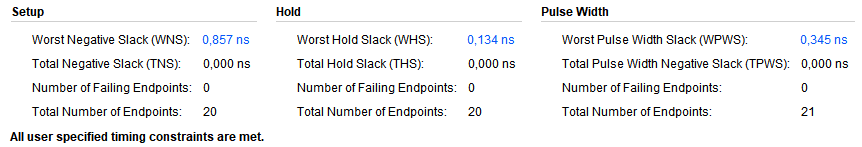
\includegraphics[scale=0.7]{img/vivado/timing_summary3.png}
	\caption{Design Timing Summary with period clock equal to 2.5 ns}
\end{figure}

\noindent We can reduce also now the clock period but, in order to have a bit margin of error (after the implementation the slack will be smaller than this value), we maintain this clock period. In any case, in order to achieve a theoretical limit to the maximum clock frequency, we obtain that, repeating this procedure, we arrive at the point that the minimum clock period is 2.2 ns and so the maximum clock frequency achievable is 454 MHz.
%\newpage
\subsection{I/O Planning}
The next step is to do the I/O planning: this means that we have to connect our inputs and our outputs to the pins of the board. We can see it in the figure 5.7.
\begin{figure}[htpb]
	\centering
	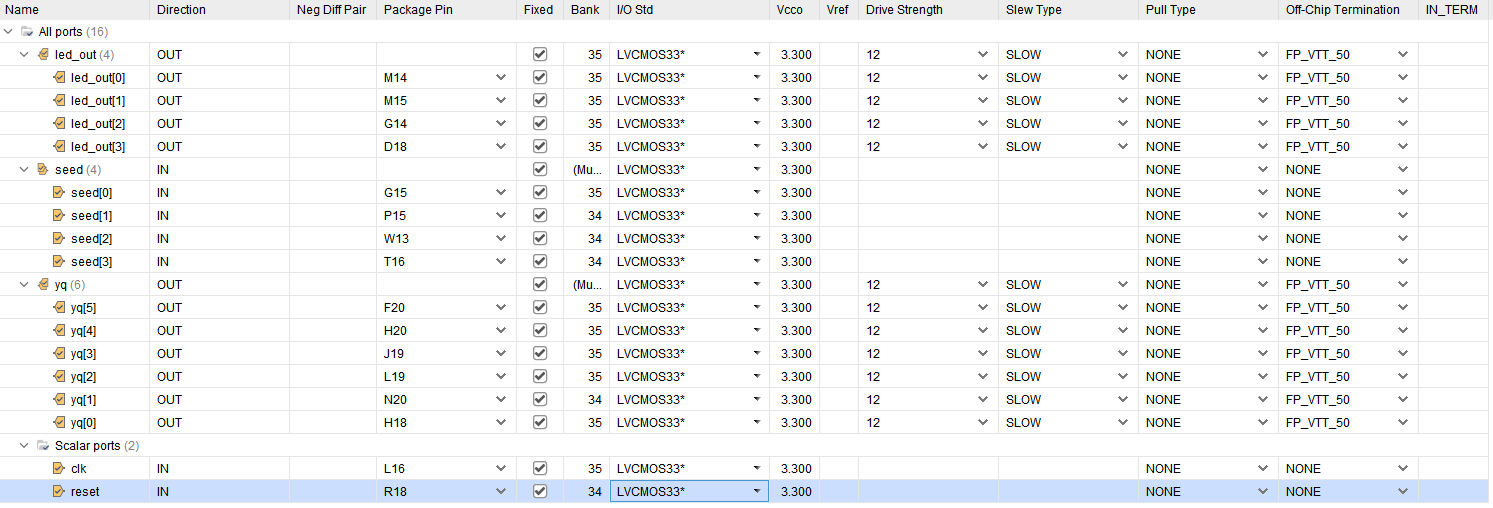
\includegraphics[scale=0.4]{img/vivado/ioplanning.png}
	\caption{I/O Planning}%\end{figure}
\end{figure}


\subsection{Warning Message Analysis}
At the end of the synthesis we have 11 warning messages. We can see them in the figure 5.8.


\begin{figure}[htpb]
	\centering
	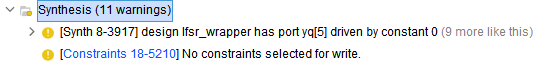
\includegraphics[scale=0.9]{img/vivado/warnings_synthesis.png}
	\caption{Warning messages after synthesis}
\end{figure}

\noindent The warning messages can be easily explained: they are related to the fact that we connect part of the output to the constant 0. But this is what we want, because we have only a bit as output and if we want to use the VGA then the other bits must be setted manually to 0, because only the LSB of \emph{yq} is the real output.

\newpage

\subsection{Estimated Resources Utilization}
The estimated resources utilized are shown in the figure 5.9 and 5.10.

\begin{figure}[htpb]
	\centering
	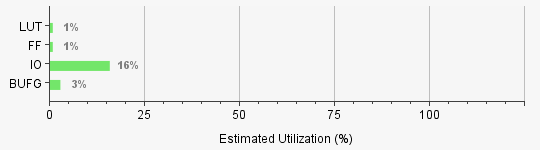
\includegraphics[scale=0.9]{img/vivado/estimated_utilization1.png}
	\caption{Graph representation of the estimated resource utilization}
\end{figure}


\noindent In the figure 5.9 we can see that the most estimated utilization is about the I/O resource, instead we use a very low number of the available flip-flops and LUTs.

\begin{figure}[htpb]
	\centering
	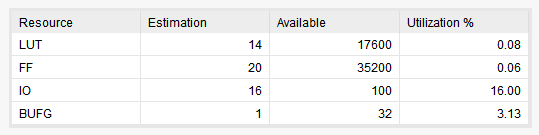
\includegraphics[scale=0.9]{img/vivado/estimated_utilization2.png}
	\caption{Table representation of the estimated resource utilization}
\end{figure}


\noindent In particular we can see in the figure 5.10 that we use 32 flip-flops and 14 LUTs with an utilization that is less than 0.1\%



\subsection{Schematic after synthesis}
After the synthesis we can see a schematic of the LFSR mapped on the target technology, so we can see how our logic is translated in terms of flip-flops and LUTs. In the figure 5.11 we can see the schematic after synthesis and in the figure 5.12 the detail of a flip flop.
\begin{figure}[htpb]
	\centering
	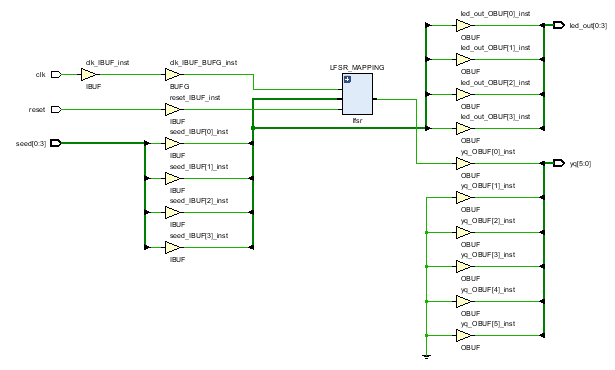
\includegraphics[scale=0.8]{img/vivado/schematic_after_synthesis.png}
	\caption{Schematic after synthesis}
\end{figure}
\begin{figure}[htpb]
	\centering
	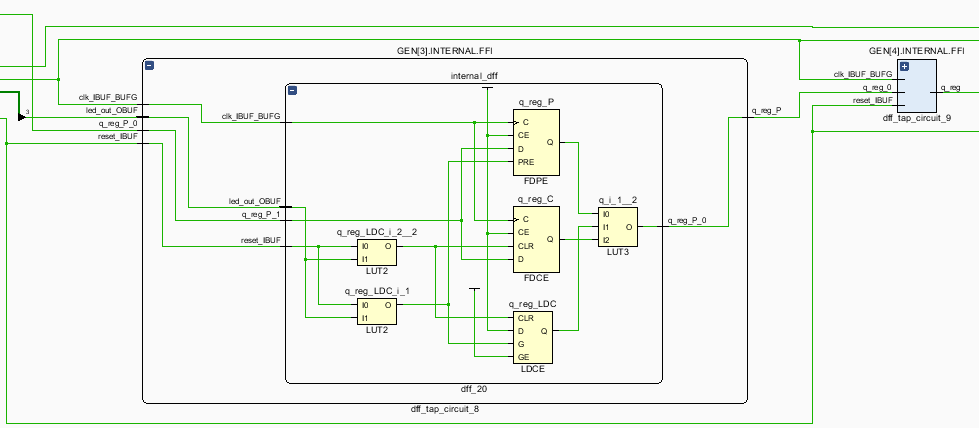
\includegraphics[scale=0.6]{img/vivado/detail_of_schematic_after_synthesis.png}
	\caption{Detail of a D-Flip-Flop with tap circuit in the schematic after synthesis}
\end{figure}

\section{Implementation}
With this phase we implement our device on the FPGA board. The previous information are estimated, now, in this phase, we have the real informations about timing, power consumption and resource utilization. So in this section we will compare the actual results with the estimate ones in order to discuss the performance of the implemented LFSR on the ZyBo Board.

\noindent As first step we can see how our functionalities are mapped on the board in the figure 5.13 where the used components are the ones in light blue.

\begin{figure}[htpb]
	\centering
	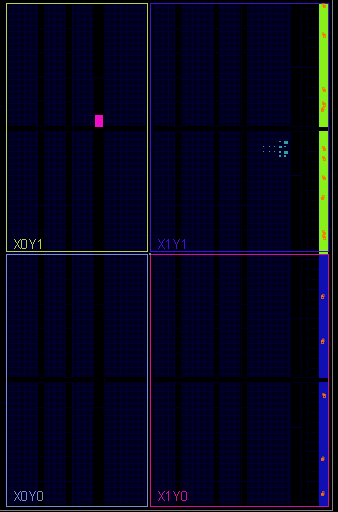
\includegraphics[scale=0.76]{img/vivado/fpga.png}
	\caption{Image that describes how our device is mapped on the FPGA}
\end{figure}

\noindent In the figure 5.14 we can see a more detailed view of some of the components used in the FPGA to implement our functionalities.

\noindent The components used are the ones in light blue, we can recognize flip-flops and LUTs.

\begin{figure}[htpb]
	\centering
	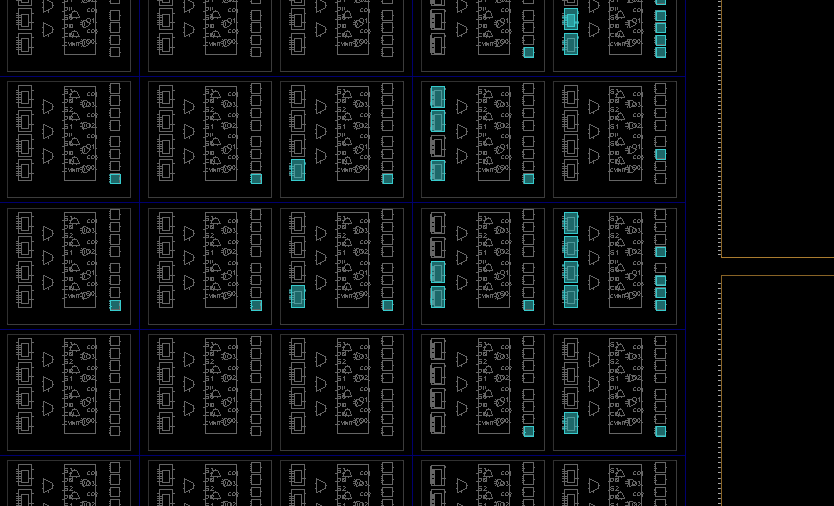
\includegraphics[scale=0.6]{img/vivado/fpga_detail.png}
	\caption{Detail of the FPGA board}
\end{figure}

\subsection{Timing Constraint}
The time constraint are respected also after the implementation. The slack is positive and so we are sure that our device can work at a frequency of 400 MHz. We can see the timing report after the implementation in the figure 5.15.

\begin{figure}[htpb]
	\centering
	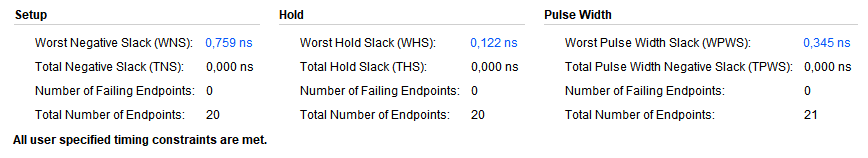
\includegraphics[scale=0.7]{img/vivado/implementation_timing.png}
	\caption{Timing report after implementation}
\end{figure}

\noindent If we try to run the implementation with the previously estimated minimum clock period (2.2ns) we have that the timing constraint are met also in this case and so the minimum clock period achievable is 2.2ns (454 MHz) but in any case we will work with the clock period equal to 2.5ns (400 MHz)
\subsection{Resources Utilization}
The utilized resources are exactly the ones estimated in the previous phase as we expect. We can see them in the figure 5.16.
\begin{figure}[htpb]
	\centering
	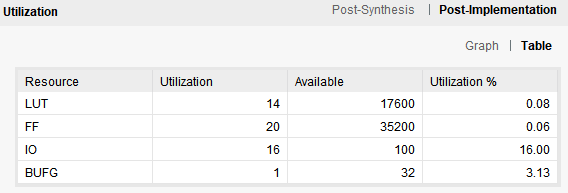
\includegraphics[scale=0.7]{img/vivado/utilization.png}
	\caption{Resource utilized after implementation}
\end{figure}

\subsection{Power Consumption}
The report for the power consumption of the programmed board is in figure 5.17.
\begin{figure}[htpb]
	\centering
	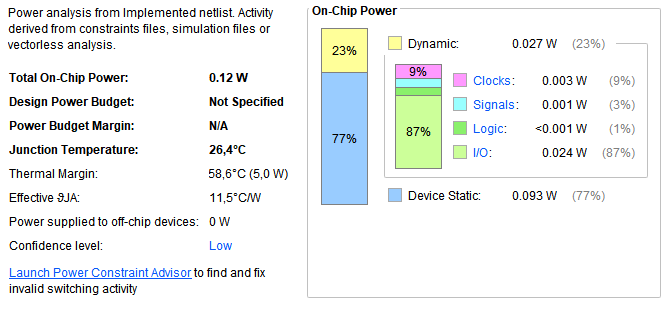
\includegraphics[scale=0.85]{img/vivado/power.png}
	\caption{Power Consumption Report}
\end{figure}

\noindent From the figure we can see that the most power consumption is static, so it is due to the fact that the device is connected to the power supply. The part of the power consumed from the switching activity is equal to 23\% and the most part of this is due to the I/O operations (87\% of the dynamic power). So, a possible solution to reduce the power consumption of the device, is to have a pre-defined seed without the possibility of changing it. But if we do this, we reduce drastically the features of the device and the possibility to generate different streams of bits (because if we maintain the same seed the stream of bits remain the same and it will be repeated after each cycle). So we can say that this power consumption is acceptable.
 
\chapter{Conclusion}
The result of this project is a Linear Feedback Shift Register implemented programming the ZyBo Board. The LFSR has a feedback polynomial equal to (if the target board would have more inputs, the LFSR can work with any feedback polynomial on less than 16 bits):
\[1+x^{11}+x^{13}+x^{14}+x^{16}\]
The architecture choosen is Galois for the performance reason explained in the section 1.4.
The LFSR can be initialized with $2^4$ possible values due to the limitations placed by the inputs of the ZyBo, otherwise it would be possible to initialize it wit $2^{16}$ possible seeds.

\noindent The output is a bit and it is given to the real world through the VGA port of the ZyBo board.

\noindent From the viewpoint of the performance, the device implemented on the ZyBo works with a clock frequency equal to 400 MHz but in theory the maximum clock frequency is 454 MHz.

\noindent About the power consumption, the device has a power equal to 0,12 W but onyly 0.027 W are due to the LFSR implementation. The utilized resource are very low and they reach a great value only for the I/O resources.

\noindent The ZyBo board, with this implemented LFSR, can be used for the application seen in the section 1.3, from the Cryptography to Communications and so on.
\end{document}
